% !TeX spellcheck = es_VE
% !TeX root = Informe.tex
% !TeX spellcheck = es_VE
\documentclass[12pt,letterpaper]{article}
\usepackage[utf8]{inputenc}
\usepackage{amsmath}
\usepackage{amsfonts}
\usepackage{amssymb}
\usepackage{graphicx}
\usepackage{url}
\usepackage{tikz}
\usepackage[shortlabels]{enumitem} % Se mantiene aquí con sus opciones
\usepackage{fancyhdr}
\usepackage[spanish]{babel}
%\usepackage[acronym]{glossaries}
%\makeglossaries

% agregar circuitos electronicos
\usepackage[siunitx, american]{circuitikz}

% comas sencillas en listing
\usepackage{textcomp}
\usepackage{upquote}
\usepackage{listings}
\lstset{upquote=true}

% dimensiones de pagina
\usepackage[left=1.5cm,top=1.5cm,right=1.5cm,bottom=2.5cm]{geometry}

% hiperenlaces
\usepackage{hyperref} % Para incluir hipervínculos
\hypersetup{urlcolor=blue,colorlinks=false,pdfborder={0 0 0}} % eliminar marco rojo en enlaces (citas, indices, pies de pagina, etc)

% permitir en la numeracion de los items agregar el numero de seccion
% (Se eliminó la línea duplicada \usepackage{enumitem} que causaba el error)
\setlist[enumerate]{label=\thesection.\arabic*. }   % numerar solo con seccion
%\setlist[enumerate]{label=\thesubsection.\arabic*. } % incluir numeracion de subsection

% otras configuraciones
\usepackage{parskip}
\setlength{\parskip}{1em} % establece el espacio entre parrafos
\setlength{\parindent}{0cm} % elimina la sangria inicial en parrafo
\usepackage{array} % ajustes adicionales para tablas
% \usepackage{pdfpages} %incluir archivos pdf en documento

% personalizacion de etiquetas
\renewcommand{\figurename}{Figura}
\renewcommand{\contentsname}{Contenido}
\renewcommand{\listfigurename}{Índice de Figuras}
\renewcommand{\listtablename}{Índice de Tablas}
\renewcommand{\lstlistlistingname}{Índice de Códigos}
\renewcommand{\tablename}{Tabla}
\renewcommand{\lstlistingname}{Código}

% pie de pagina
\renewcommand{\footrulewidth}{0.4pt}% grosor de linea del pie de pag
%\lfoot{\thepage} % texto izquierda
%\rfoot{\thepage} % texto derecha
\cfoot{\thepage} % texto al centro

%% definiciones para insertar codigo de programacion al doc
\usepackage{color}
\definecolor{dkgreen}{rgb}{0,0.6,0}
\definecolor{gray}{rgb}{0.5,0.5,0.5}
\definecolor{mauve}{rgb}{0.58,0,0.82}
\lstset{frame=tb,
    language=Python,
    aboveskip=3mm,
    belowskip=3mm,
    showstringspaces=false,
    columns=flexible,
    basicstyle={\small\ttfamily},
    %numbers=left,
    numberstyle=\tiny\color{gray},
    keywordstyle=\color{blue},
    commentstyle=\color{dkgreen},
    stringstyle=\color{mauve},
    breaklines=true,
    breakatwhitespace=true,
    tabsize=3
} % fin de codigo de programacion

%%%%%%%%%%%%%% MACRO PARA CONTROL DE PUNTAJE %%%%%%%%%%%%%%%%%%
\usepackage{xifthen}
\newcounter{puntos}
\setcounter{puntos}{0} % Inicializa el contador a cero

\newcommand{\sumarPunto}[1]{%
    \addtocounter{puntos}{#1}%
    \ifthenelse{#1 > 1}{(\textbf{#1 puntos})}{(\textbf{#1 punto})} 
}
%%%%%%%%%%%%%%%%%%%%%%%%%%%%%%%%%%%%%%%%%%%%%%%%%%%%%%%%%%
\usepackage[T1]{fontenc}

%%%%%%%%%%%%%%%%%%%%%%%%%%%%%%%%%%%%%%%%%%%%%%%%%%%%%%%%%%%%%%%%%%%%%%%
\pagestyle{fancy}
\fancyhf{}

\setlength{\headheight}{80pt}
\addtolength{\topmargin}{-35pt}
\setlength{\headsep}{1cm}
\setlength{\footskip}{20pt}

\rhead{
\includegraphics[width=1.3cm]{../img/logo_ciencias.png}}
\lhead{
\includegraphics[width=1.4cm]{../img/logo_ucv.png}}
\cfoot{\thepage}
\rfoot{Junio, 2026}

\chead{Laboratorio de Internet de las Cosas}
\newcommand{\titulo}{LABORATORIO 3}
\newcommand{\subtitulo}{Interfaz Gr\'{a}fica con Processing y Protocolo Firmata}
\newcommand{\autorUno}{Luisdavid Colina V24766381}
\newcommand{\autorDos}{Samantha Ram\'{i}rez V31307714}
%%%%%%%%%%%%%%%%%%%%%%%%%%%%%%%%%%%%%%%%%%%%%%%%%%%%%%%%%%%%%%%%%%%%%%%
\begin{document}

%%%%%%%%%%%%%%%%%%%%%%%%%%%%%%%%%%%%%%%%%%%%%%%%%%%%%%%%%%%%%%%%%%%%%%%
\begin{center}
  {\Large \textbf{\titulo}} \\[0.3cm]
  {\large \textbf{\subtitulo}} \\[0.8cm]

  \small
  \begin{tabular}{c}
    \textbf{Preparado por:} \\
    \autorUno \\
    \autorDos \\
  \end{tabular}
  \\[1cm]
\end{center}

%%%%%%%%%%%%%%%%%%%%%%%%%%%%%%%%%%%%%%%%%%%%%%%%%%%%%%%%%%%%%%%%%%%%%%%
\section{Desarrollo de actividades}

\subsection{Actividad 5.1: Carga del firmware StandardFirmata}
\textit{Enunciado: Compile y suba a la placa el c\'{o}digo StandardFirmata disponible en la
secci\'{o}n de ejemplos del IDE de Arduino.}

Firmata es un protocolo que permite controlar los pines del Arduino desde un programa
externo en el computador sin tener que reprogramar la placa cada vez~\cite{firmata}.
Para cargarlo, en el IDE se seleccionó \emph{Archivo} $\to$ \emph{Ejemplos} $\to$ \emph{Firmata} $\to$
\emph{StandardFirmata} y se subi\'{o} a la placa por USB. Con eso el Arduino
queda escuchando comandos por el puerto serial y Processing puede
comunicarse con \'{e}l directamente.

\clearpage
%%%%%%%%%%%%%%%%%%%%%%%%%%%%%%%%%%%%%%%%%%%%%%%%%%%%%%%%%%%%%%%%%%%%%%%
\subsection{Actividad 5.2: Control de LED RGB desde Processing}
\textit{Enunciado: Construya una interfaz de usuario, utilizando Processing, que permita
controlar la intensidad y el color de un led RGB conectado a la placa, los controles deben
ser de tipo \emph{slider}. Muestre un componente que represente al LED RGB y que modifique
su color conforme a los sliders. Implemente un componente que muestre los valores de los
componentes RGB y un gr\'{a}fico de intensidad de color.}

Para el circuito se conectaron las tres patas del LED RGB a los pines 3, 6 y 5 de la placa
(rojo, verde y azul), cada una con su resistencia de 220~$\Omega$. Se usaron esos pines
en particular porque tienen soporte PWM, que es lo que se necesita para variar la
intensidad de cada color. El dise\~{n}o en Fritzing se puede ver en la
Figura~\ref{fig:diseno_act1} y el montaje armado en la Figura~\ref{fig:circuito_act1}.

\begin{figure}[ht!]
    \centering
    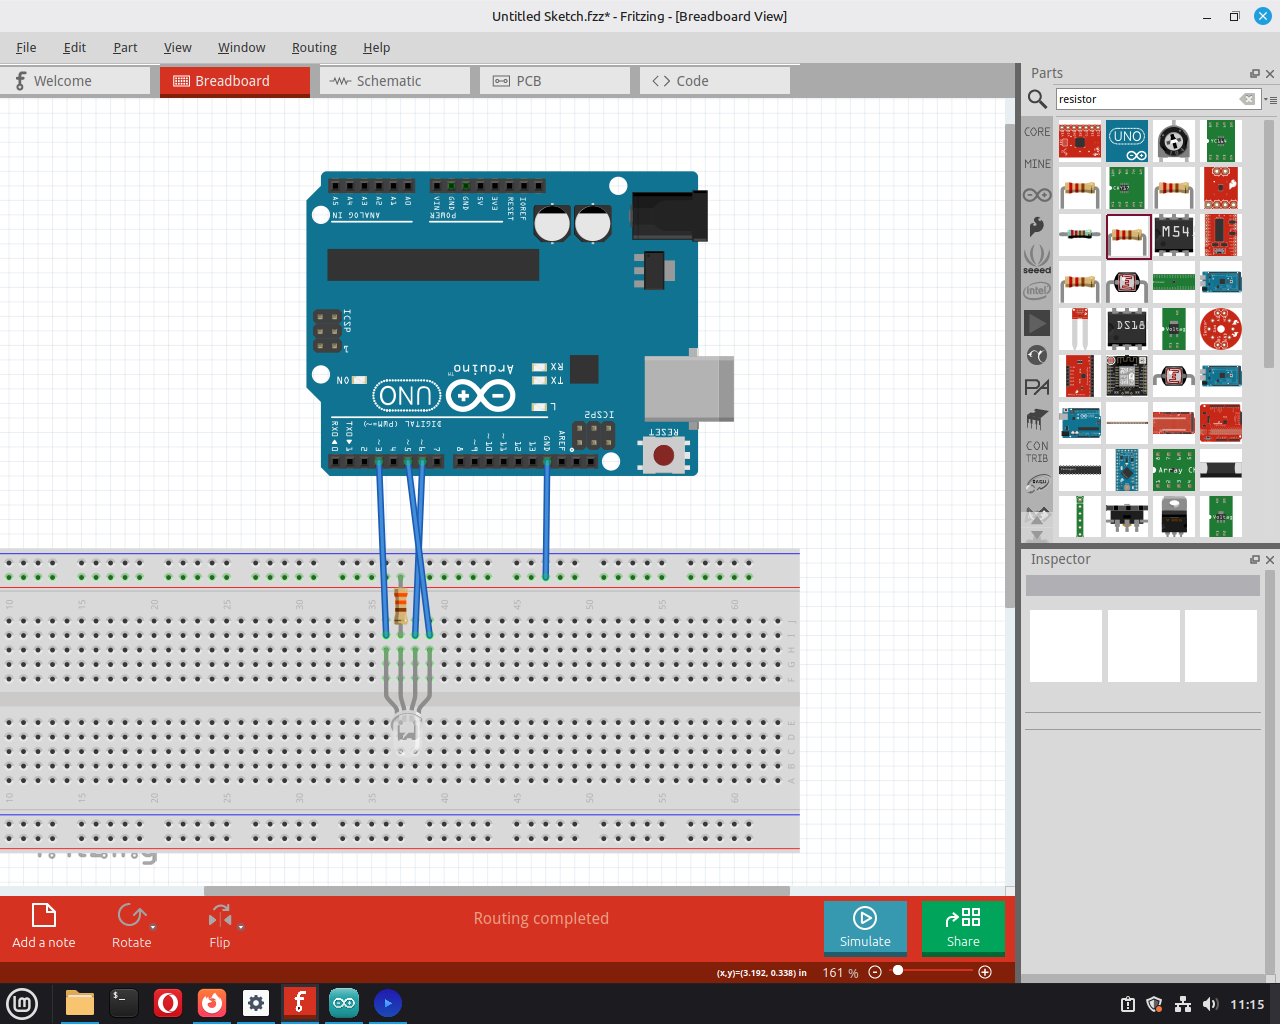
\includegraphics[width=0.8\linewidth]{img/diseno_act1.png}
    \caption{Dise\~{n}o del circuito para el LED RGB en Fritzing.}
    \label{fig:diseno_act1}
\end{figure}
\begin{figure}[ht!]
    \centering
    
\includegraphics[width=0.6\linewidth]{img/circuito_act1.jpg}
    \caption{Montaje f\'{i}sico del LED RGB sobre el protoboard.}
    \label{fig:circuito_act1}
\end{figure}

\pagebreak
La interfaz se hizo en Processing usando las librer\'{i}as \texttt{controlP5} (para los
controles de la pantalla) y \texttt{cc.arduino} (para hablar con la placa por Firmata).
Lo primero fue declarar los pines y configurarlos como salida
(C\'{o}digo~\ref{lst:pin_setup}):

\begin{lstlisting}[language=Java,
    caption={Declaraci\'{o}n de pines y configuraci\'{o}n en \texttt{setup()}.},
    label={lst:pin_setup}, 
    float=ht!]
int ledRojo = 3;
int ledVerde = 6;
int ledAzul  = 5;

arduino = new Arduino(this, Arduino.list()[2], 57600);
arduino.pinMode(ledRojo, Arduino.OUTPUT);
arduino.pinMode(ledVerde, Arduino.OUTPUT);
arduino.pinMode(ledAzul,  Arduino.OUTPUT);
\end{lstlisting}

Los tres sliders se crearon usando \texttt{cp5.addSlider()} con rango de 0 a 255, que es el
rango del PWM en 8 bits (C\'{o}digo~\ref{lst:sliders}). Tambi\'{e}n se agreg\'{o} un
gr\'{a}fico de l\'{i}nea para mostrar el historial de intensidad.

\begin{lstlisting}[language=Java,
    caption={Creaci\'{o}n de sliders y gr\'{a}fico en \texttt{setup()}.},
    label={lst:sliders}, 
    float=ht!]
cp5.addSlider("slider1").setPosition(50,  50).setRange(0, 255).setSize(150, 20);
cp5.addSlider("slider2").setPosition(50, 110).setRange(0, 255).setSize(150, 20);
cp5.addSlider("slider3").setPosition(50, 170).setRange(0, 255).setSize(150, 20);

myChart1 = cp5.addChart("ledVerde")
              .setPosition(50, 200).setSize(200, 100)
              .setRange(0, 255).setView(Chart.LINE).setStrokeWeight(1.5);
myChart1.addDataSet("incoming");
myChart1.setData("incoming", new float[100]);
\end{lstlisting}

\pagebreak
En \texttt{draw()} se lee el valor de cada slider y se manda al pin correspondiente con
\texttt{analogWrite()}. Tambi\'{e}n se llama a \texttt{dibujarLED()} para mostrar en
pantalla el estado del LED, y se actualiza el gr\'{a}fico cada 5 frames para que no sea
tan pesado (C\'{o}digo~\ref{lst:draw_rgb}). La funci\'{o}n \texttt{dibujarLED()} usa el
alfa del color para que el c\'{i}rculo en pantalla sea m\'{a}s o menos brillante seg\'{u}n
el valor del slider, igual que el LED f\'{i}sico (C\'{o}digo~\ref{lst:led_draw}).

\begin{lstlisting}[language=Java,
    caption={Lectura de sliders, escritura en pines y actualizaci\'{o}n visual en
    \texttt{draw()}.},
    label={lst:draw_rgb}, 
    float=ht!]
int valorSlider1 = (int)cp5.getController("slider1").getValue();
int valorSlider2 = (int)cp5.getController("slider2").getValue();
int valorSlider3 = (int)cp5.getController("slider3").getValue();

arduino.analogWrite(ledRojo, valorSlider1);
arduino.analogWrite(ledVerde, valorSlider2);
arduino.analogWrite(ledAzul,  valorSlider3);

dibujarLED(260,  60, color(255, 0, 0), valorSlider1);
dibujarLED(260, 120, color(0, 255, 0), valorSlider2);
dibujarLED(260, 180, color(0, 0, 255), valorSlider3);

if (frameCount % 5 == 0)
    myChart1.push("incoming", valorSlider3);
\end{lstlisting}

\begin{lstlisting}[language=Java,
    caption={Funci\'{o}n para dibujar el LED virtual en pantalla.},
    label={lst:led_draw}, 
    float=ht!]
void dibujarLED(int x, int y, color c, int val) {
    fill(red(c), green(c), blue(c), val);
    noStroke();
    ellipse(x, y, 40, 40);
    stroke(255, 50);
    noFill();
    ellipse(x, y, 30, 30);
}
\end{lstlisting}

Adem\'{a}s se implement\'{o} un panel que muestra en tiempo real los valores de los tres
canales y la fotorresistencia (C\'{o}digo~\ref{lst:panel_valores}).

\begin{lstlisting}[language=Java,
    caption={Panel de valores en tiempo real.},
    label={lst:panel_valores},
    float=ht!]
void dibujarVentanaValores(int x, int y, int w, int h) {
    fill(0, 0, 0, 150);
    stroke(255, 100);
    rect(x, y, w, h, 10);
    fill(0, 255, 0);
    textSize(12);
    text("DATOS EN TIEMPO REAL", x + 10, y + 20);
    fill(255);
    textSize(14);
    text("Led Rojo:        " + nf(cp5.getController("slider1").getValue(), 0, 1), x+10, y+45);
    text("Led Verde:       " + nf(cp5.getController("slider2").getValue(), 0, 1), x+10, y+65);
    text("Led Azul:        " + nf(cp5.getController("slider3").getValue(), 0, 1), x+10, y+85);
    text("Fotoresistencia: " + nf(arduino.analogRead(0),                  0, 1), x+10, y+105);
}
\end{lstlisting}

En la Figura~\ref{fig:resultado_act1_interfaz} se ve la interfaz corriendo con los sliders,
los LEDs virtuales, el panel de valores y el gr\'{a}fico. La
Figura~\ref{fig:resultado_act1_led} muestra el LED f\'{i}sico encendido con el color que
se le estaba mandando desde la interfaz.

\begin{figure}[ht!]
    \centering
    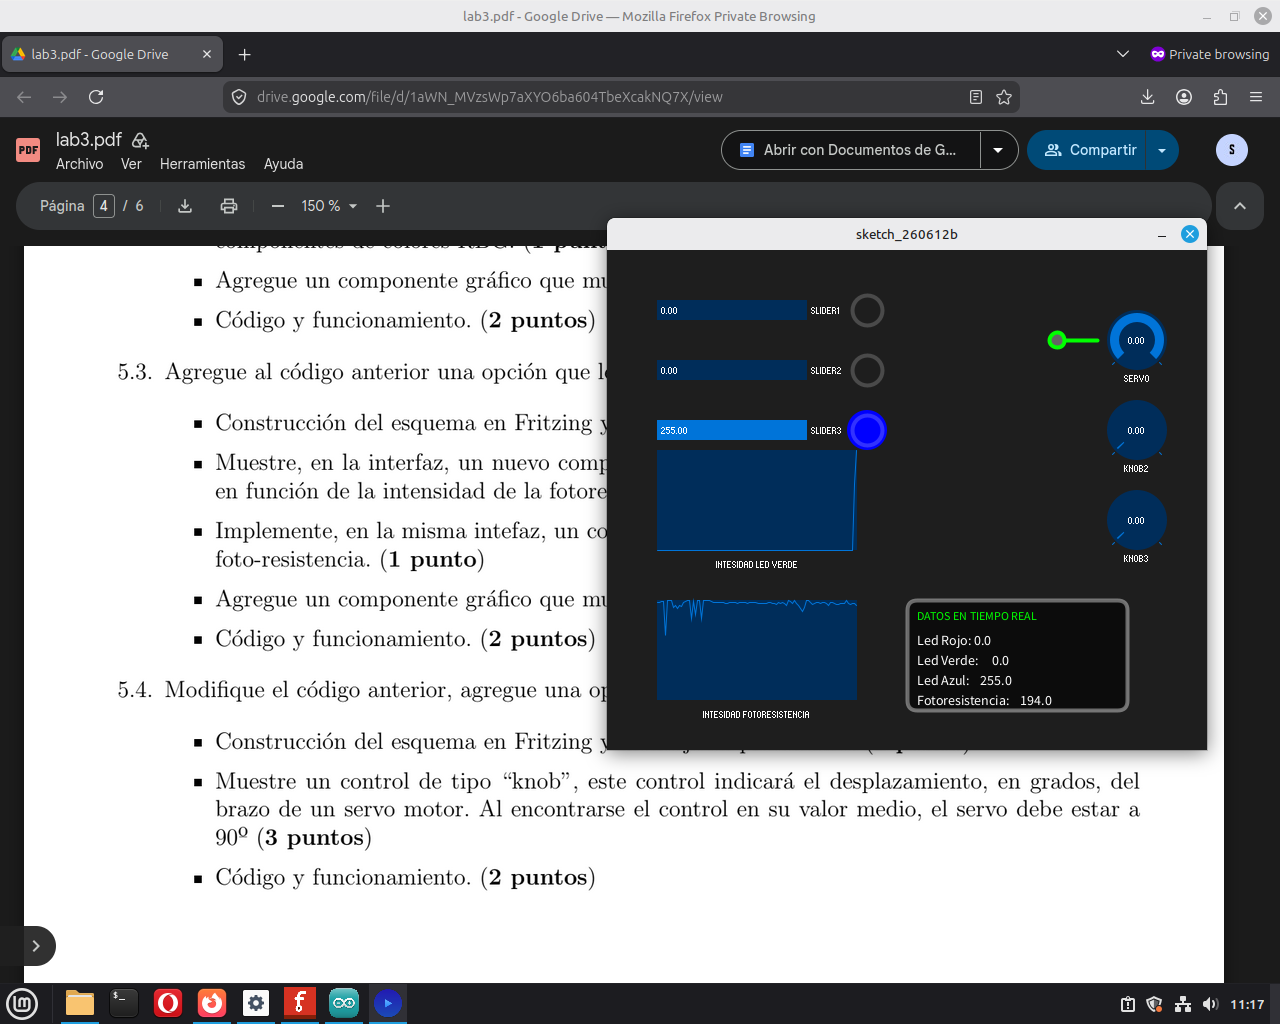
\includegraphics[width=0.8\linewidth]{img/resultado_act1_interfaz.png}
    \caption{Interfaz en ejecuci\'{o}n: sliders, LEDs virtuales, panel de valores y gr\'{a}fico.}
    \label{fig:resultado_act1_interfaz}
\end{figure}
\begin{figure}[ht!]
    \centering
    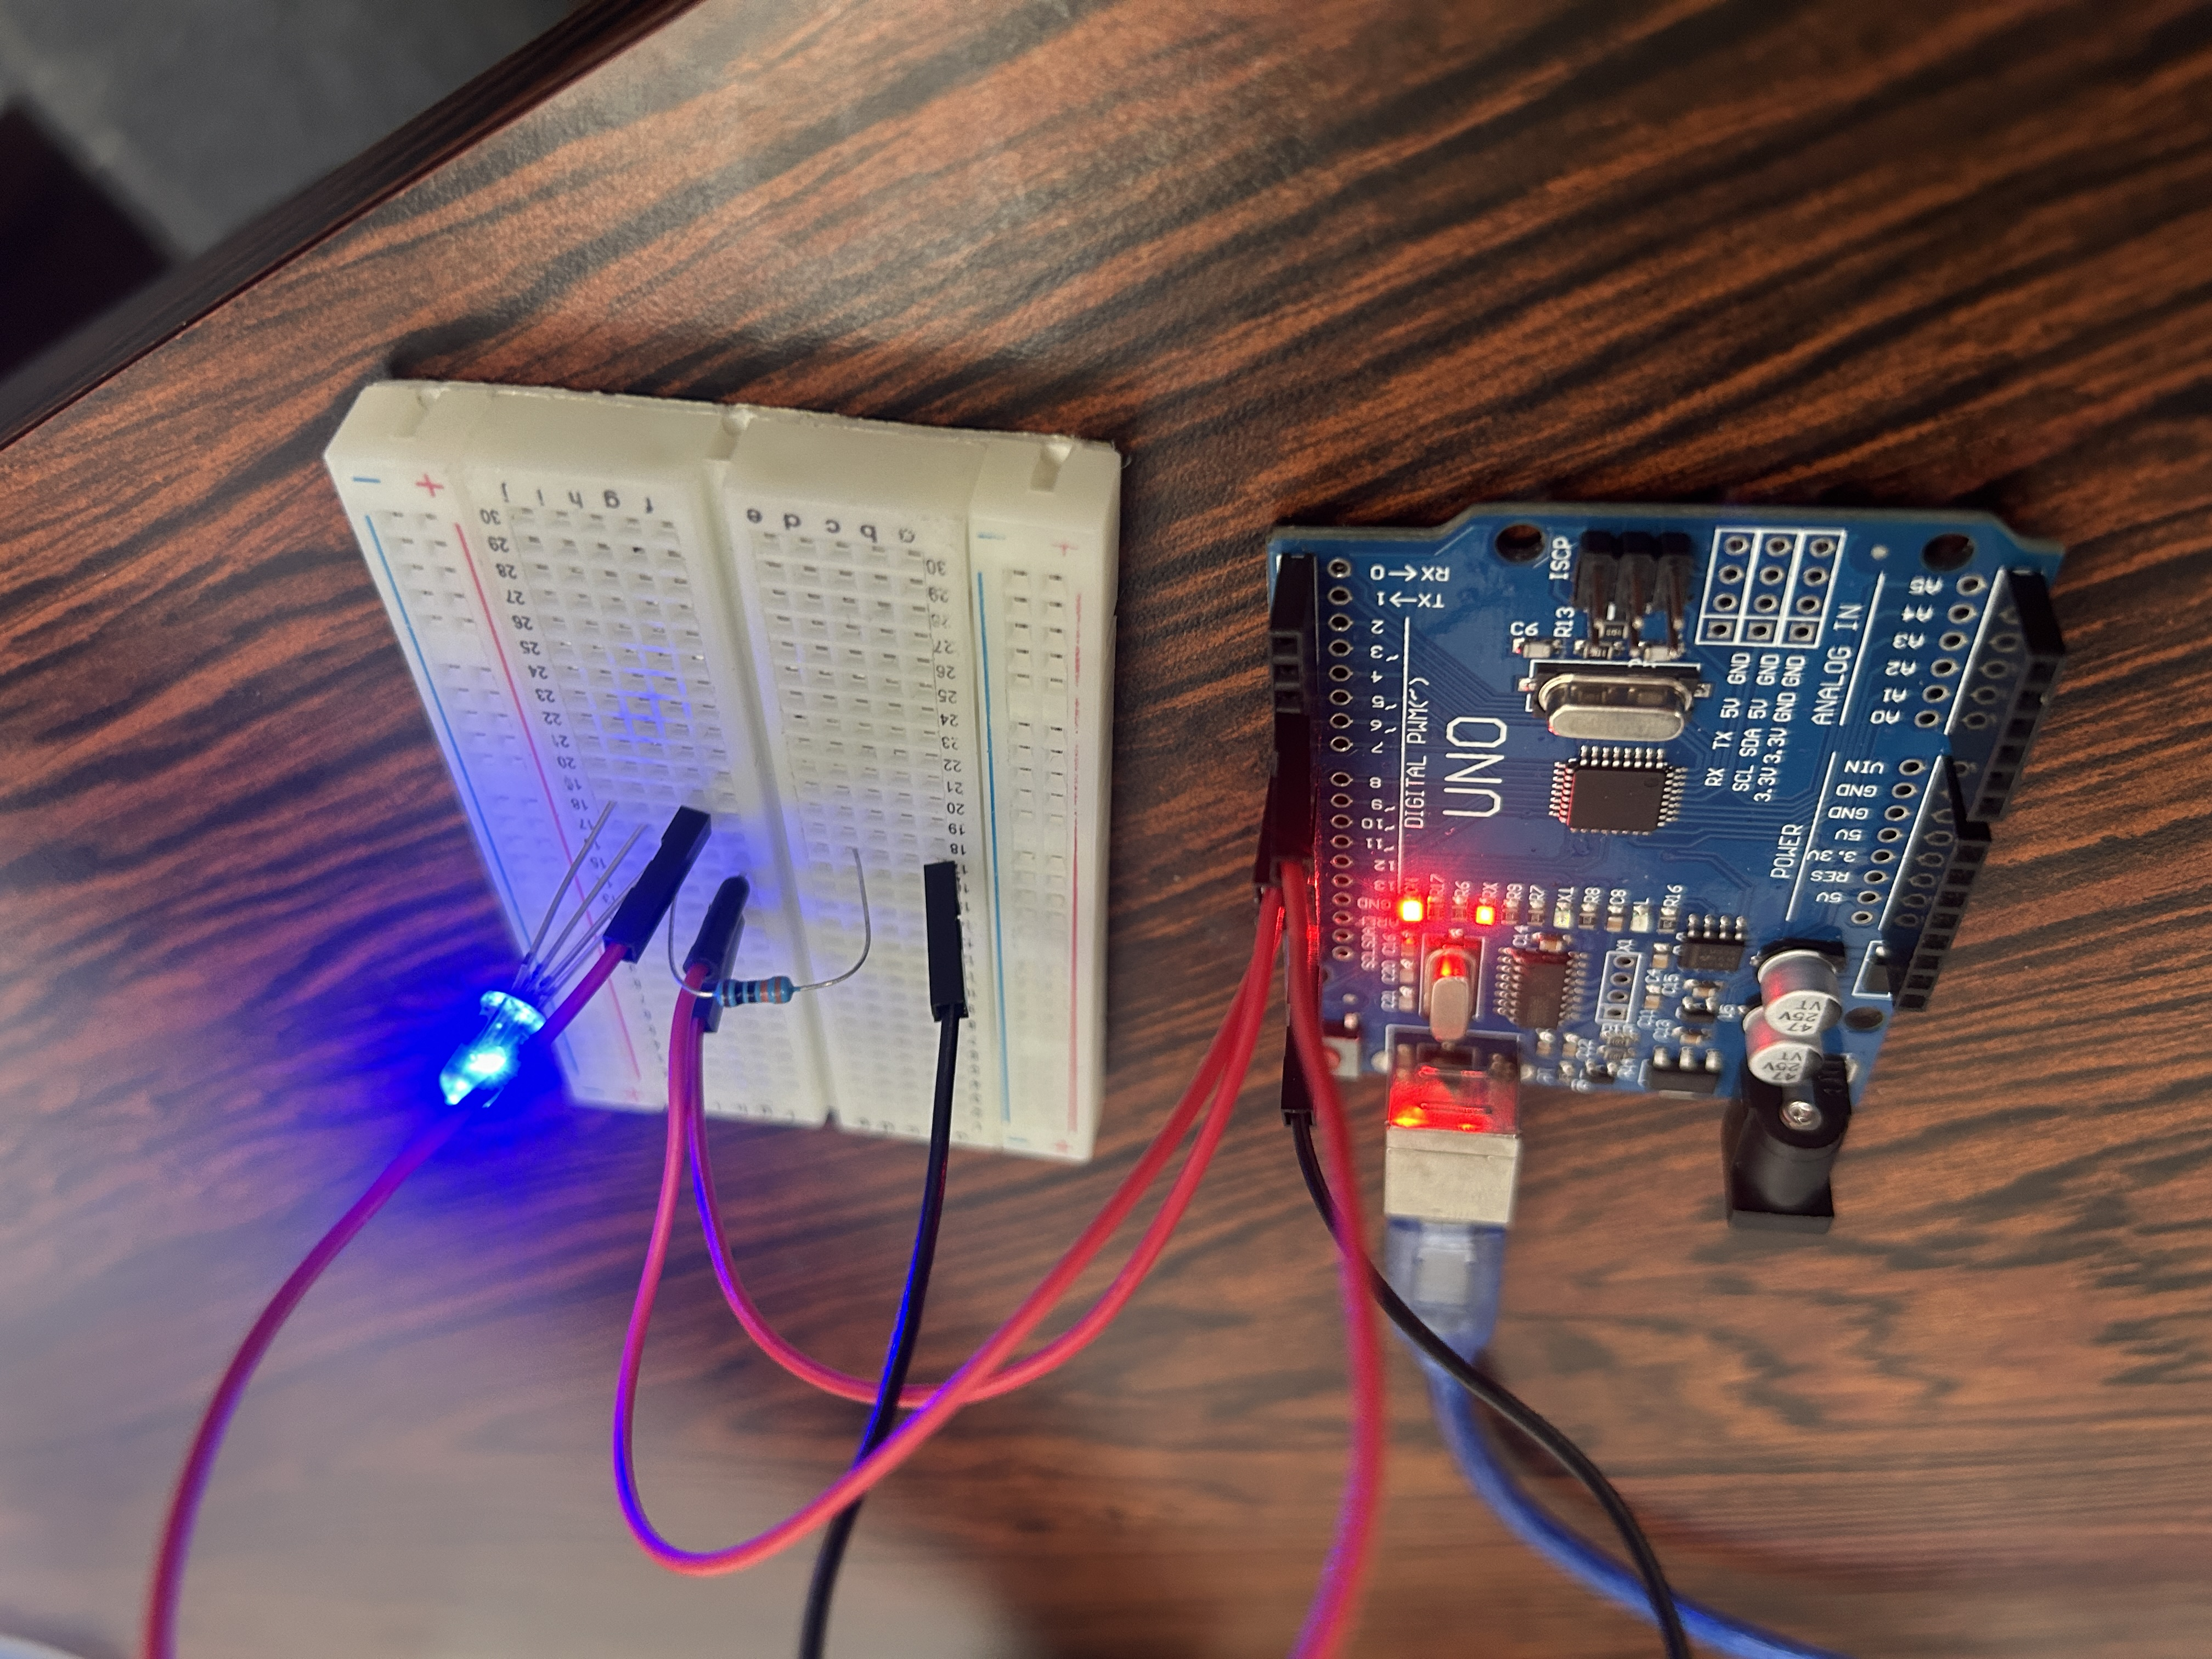
\includegraphics[width=0.5\linewidth]{img/resultado_act1_led.jpg}
    \caption{LED RGB encendido f\'{i}sicamente con el color definido en la interfaz.}
    \label{fig:resultado_act1_led}
\end{figure}

\clearpage
%%%%%%%%%%%%%%%%%%%%%%%%%%%%%%%%%%%%%%%%%%%%%%%%%%%%%%%%%%%%%%%%%%%%%%%
\subsection{Actividad 5.3: Lectura de fotorresistencia}
\textit{Enunciado: Agregue al código anterior una opción que lea valores de una 
foto-resistencia. Muestre, en la interfaz, un nuevo componente tipo led monocromático y modifique su valor en función 
de la intensidad de la fotoresistencia. Implemente, en la misma interfaz, un componente que 
muestre los valores de intensidad de la foto-resistencia. Agregue un componente gráfico que 
muestre la intensidad del fotoresistor.}

Para esta actividad, se incorporó una fotoresistencia al circuito que ya se venía trabajando. Se armó un divisor de tensión básico: conectamos una pata del componente a los 5V y la otra al pin analógico A0 del Arduino, colocando también una resistencia de protección que va hacia tierra (GND). De esta forma, podemos medir cómo cambia el voltaje dependiendo de la cantidad de luz que recibe el sensor. El diseño del circuito en Fritzing se puede ver en la Figura~\ref{fig:diseno_act2}, y el montaje real armado en el protoboard se muestra en la Figura~\ref{fig:circuito_act2}.

\begin{figure}[ht!]
    \centering
    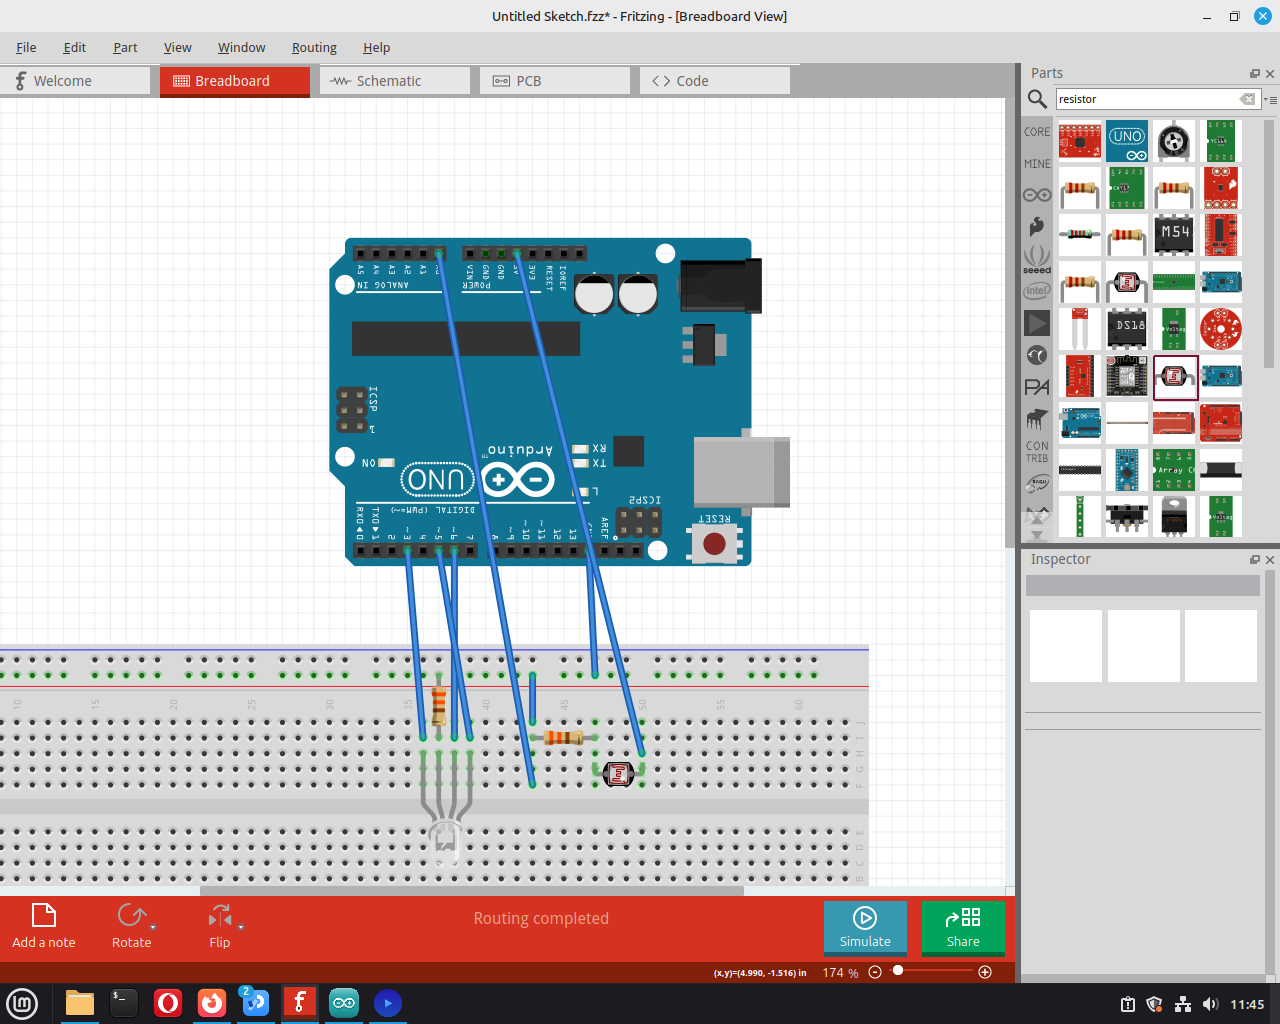
\includegraphics[width=0.8\linewidth]{img/diseno_act2.png}
    \caption{Dise\~{n}o del circuito para la fotoresistencia en Fritzing.}
    \label{fig:diseno_act2}
\end{figure}
\begin{figure}[ht!]
    \centering
    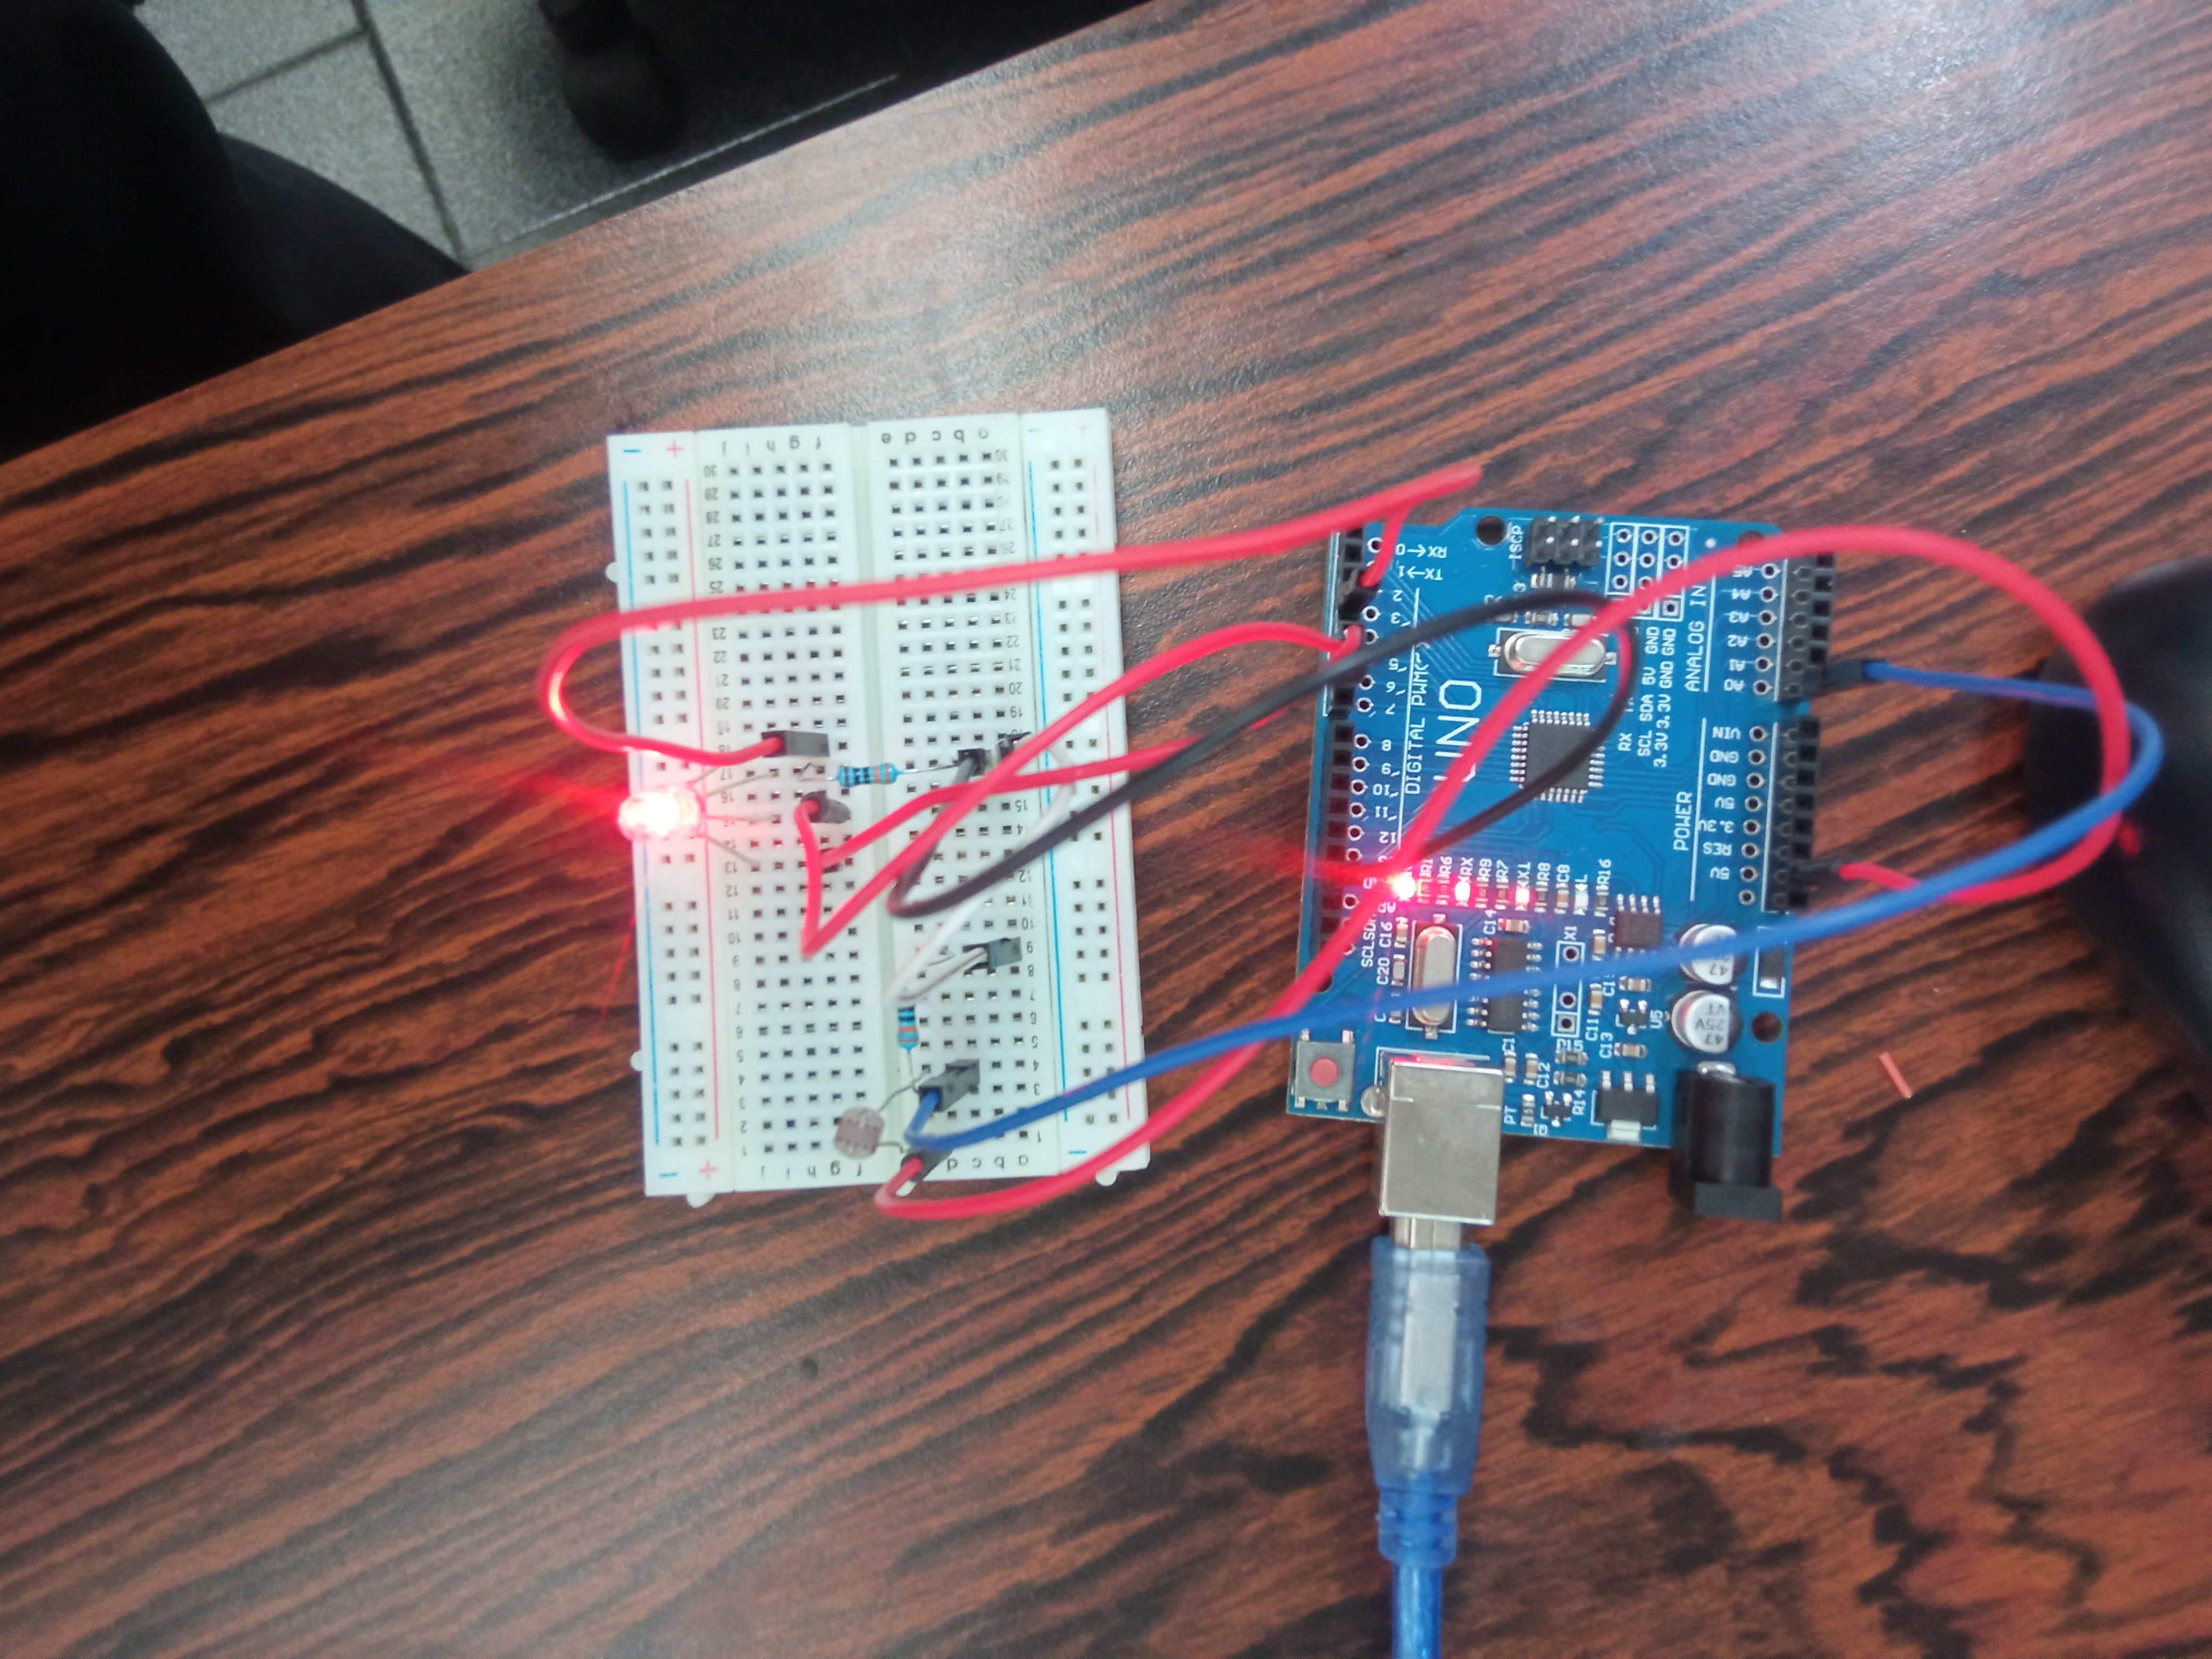
\includegraphics[width=0.6\linewidth]{img/circuito_act2.jpg}
    \caption{Montaje f\'{i}sico de la fotoresistencia sobre el protoboard.}
    \label{fig:circuito_act2}
\end{figure}

\pagebreak
En el código de Processing, se agregaron los nuevos elementos para la interfaz. En la función \texttt{setup()}, se creó un nuevo gráfico (\texttt{Chart}) para ir dibujando la línea con los valores de la luz en el tiempo, ajustando su tamaño y color para que combine con el resto de la pantalla (C\'{o}digo~\ref{lst:grafica_fotoresistencia}).

\begin{lstlisting}[language=Java,
    caption={Creación del gráfico para la fotorresistencia en \texttt{setup()}.},
    label={lst:grafica_fotoresistencia}, 
    float=ht!]

// --- Graficar valor de la Fotoresistencia ---
myChart2 = cp5.addChart("fotoresistencia")
              .setPosition(50, 350)
              .setSize(200, 100)
              .setRange(0, 200)
              .setView(Chart.LINE)
              .setStrokeWeight(1.5)
              .setColorCaptionLabel(color(40));

myChart2.addDataSet("incoming2");
myChart2.setData("incoming2", new float[100]);
\end{lstlisting}

\pagebreak
Luego, dentro de la función \texttt{draw()}, usamos \texttt{arduino.analogRead(0)} para leer el valor del pin \texttt{A0} a través de Firmata. Este se utiliza para tres cosas en la interfaz: mostrar el valor numérico en el panel de texto, enviarlo al gráfico inferior para actualizar la línea, y cambiar el nivel de transparencia de un nuevo LED virtual dibujado en pantalla (C\'{o}digo~\ref{lst:lectura_pin}).

\begin{lstlisting}[language=Java,
    caption={Lectura del pin A0 y actualización de la interfaz en \texttt{draw()}.},
    label={lst:lectura_pin}, 
    float=ht!]

float valorFotoresistencia = arduino.analogRead(0);

if (frameCount % 5 == 0) { 
    myChart2.push("incoming2", valorFotoresistencia);
}

dibujarLED(260, 240, color(0, 255, 0), (int)valorFotoresistencia);

\end{lstlisting}

Cuando la fotoresistencia recibe la iluminación normal del cuarto, el valor se mantiene estable. Para probar que la interfaz responde correctamente, tapamos el sensor físico con el dedo para bloquear la luz, como se observa en la Figura~\ref{fig:resultado_act2_fotoresistencia}. Al hacer esto, el valor de voltaje que lee el pin A0 baja rápidamente. Esto se refleja al instante en Processing: la línea del gráfico inferior cae de golpe, el número en pantalla disminuye (llegando a 11.0) y el LED virtual verde se vuelve más opaco (Figura~\ref{fig:resultado_act2_interfaz}).

\begin{figure}[ht!]
    \centering
    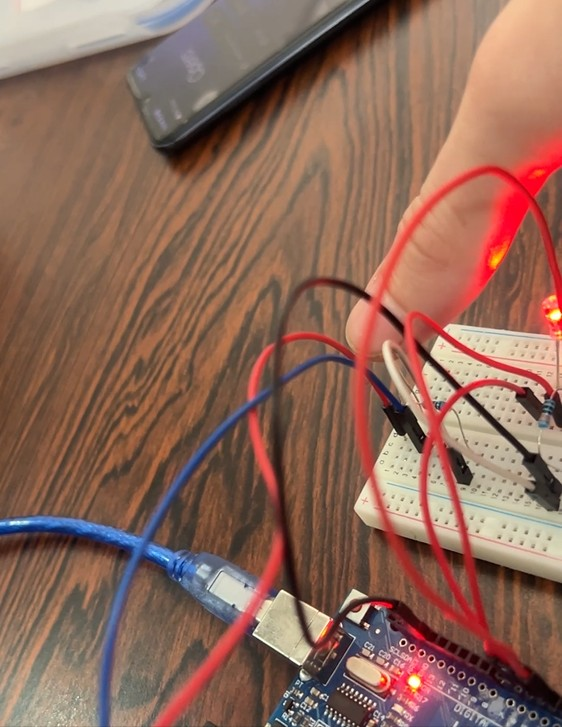
\includegraphics[width=0.4\linewidth]{img/resultado_act2_fotoresistencia.jpg}
    \caption{Bloqueo de luz en el sensor físico.}
    \label{fig:resultado_act2_fotoresistencia}
\end{figure}
\begin{figure}[ht!]
    \centering
    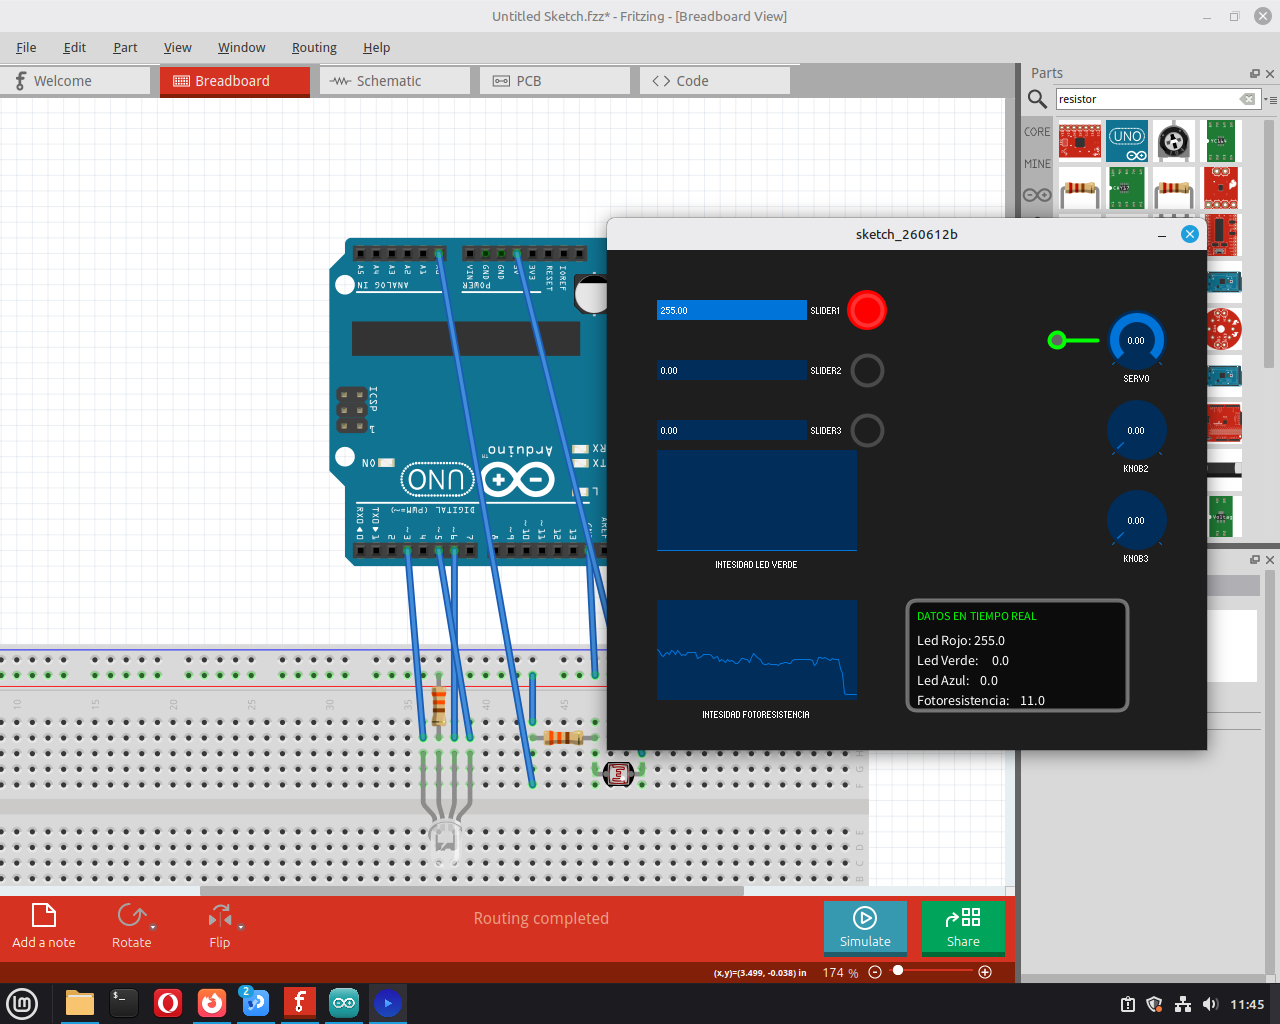
\includegraphics[width=0.6\linewidth]{img/resultado_act2_interfaz.png}
    \caption{Interfaz con gráfica de la fotoresistencia.}
    \label{fig:resultado_act2_interfaz}
\end{figure}

\clearpage
%%%%%%%%%%%%%%%%%%%%%%%%%%%%%%%%%%%%%%%%%%%%%%%%%%%%%%%%%%%%%%%%%%%%%%%
\subsection{Actividad 5.4: Control de servo motor}
\textit{Enunciado: Modifique el c\'{o}digo anterior, agregue una opci\'{o}n para controlar
un servo motor. Muestre un control de tipo \emph{knob} que indique el desplazamiento en
grados del brazo del servo. Al encontrarse el control en su valor medio, el servo debe
estar a $90^\circ$.}

Se agreg\'{o} un servo motor al circuito connect\'{a}ndolo al pin digital 10. Con
Firmata, al configurar un pin como servo, la placa genera autom\'{a}ticamente la se\~{n}al
de posicionamiento sin que Processing tenga que hacer nada extra~\cite{firmata}. El
dise\~{n}o del circuito est\'{a} en la Figura~\ref{fig:diseno_act3} y el montaje f\'{i}sico
en la Figura~\ref{fig:circuito_act3}.

\begin{figure}[ht!]
    \centering
    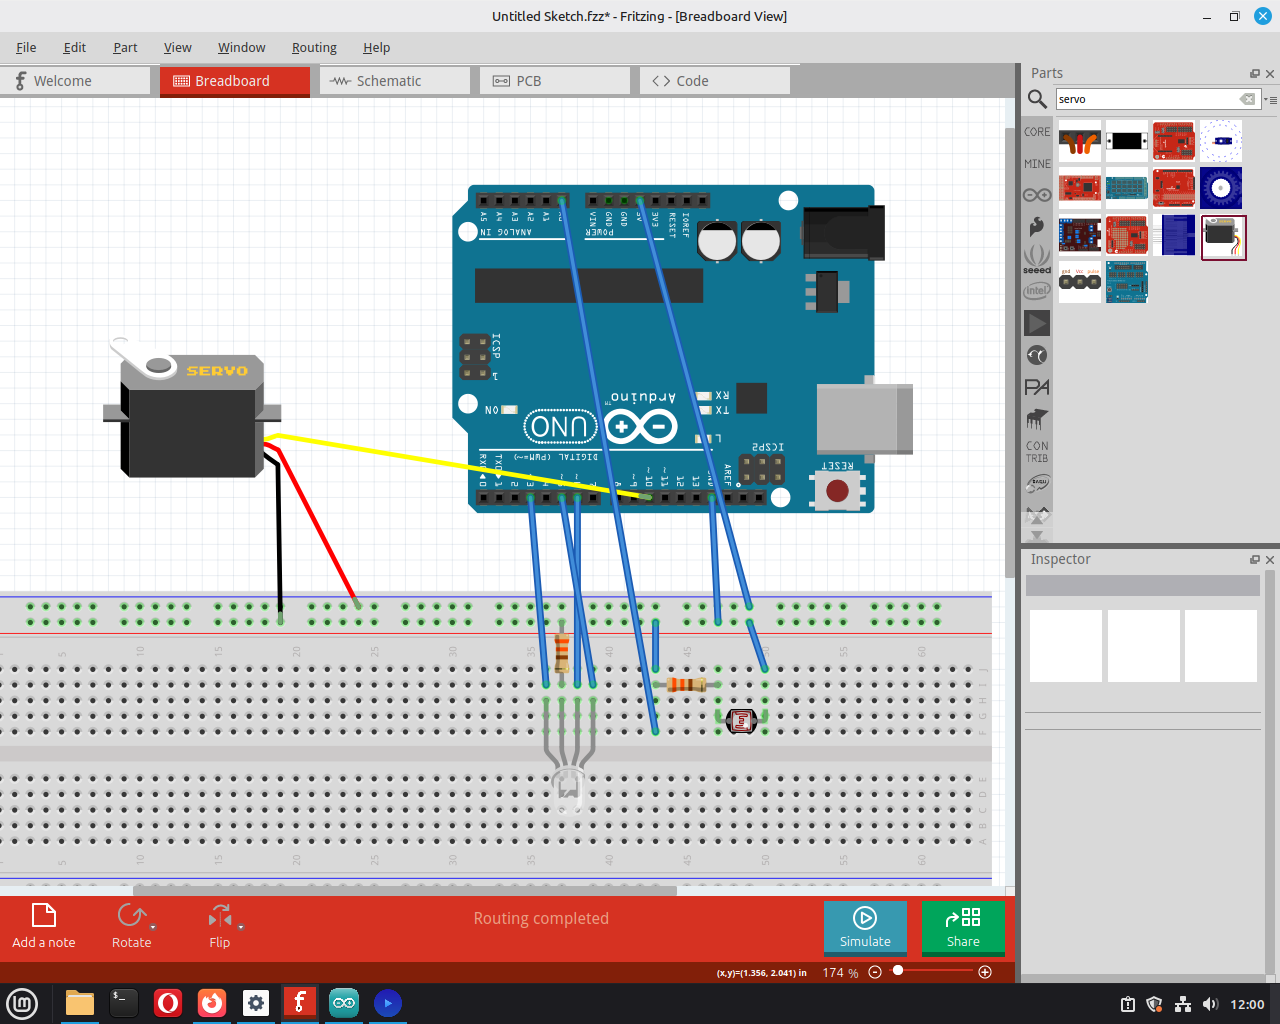
\includegraphics[width=0.8\linewidth]{img/diseno_act3.png}
    \caption{Dise\~{n}o del circuito para el servo motor en Fritzing.}
    \label{fig:diseno_act3}
\end{figure}
\begin{figure}[ht!]
    \centering
    
\includegraphics[width=0.6\linewidth]{img/circuito_act3.jpg}
    \caption{Montaje f\'{i}sico del servo motor sobre el protoboard.}
    \label{fig:circuito_act3}
\end{figure}

\pagebreak
El pin 10 se configur\'{o} con \texttt{Arduino.SERVO} para que Firmata sepa que tiene que
manejar ese pin como servo y no como salida digital normal
(C\'{o}digo~\ref{lst:servo_setup}):

\begin{lstlisting}[language=Java,
    caption={Declaraci\'{o}n y configuraci\'{o}n del pin del servo.},
    label={lst:servo_setup}, 
    float=ht!]
int servoPin = 10;
...
arduino.pinMode(servoPin, Arduino.SERVO);
\end{lstlisting}

\pagebreak
Para el knob se us\'{o} un rango de $-180$ a $0$ en lugar de $0$ a $180$
(C\'{o}digo~\ref{lst:servo_knob}). Esto se hizo para que cuando el knob est\'{e} en la
mitad su valor sea $-90$, y al multiplicarlo por $-1$ antes de mandarlo al servo queda en
$90^\circ$, que es justo lo que pide el enunciado. En \texttt{dibujarServo()} se dibuja
una l\'{i}nea que rota igual que el brazo del servo f\'{i}sico.

\begin{lstlisting}[language=Java,
    caption={Knob del servo y su control en \texttt{draw()}.},
    label={lst:servo_knob}, 
    float=ht!]
// setup():
cp5.addKnob("Servo").setPosition(500, 60).setRadius(30).setRange(-180, 0);

// draw():
int anguloServo = (int)cp5.getController("Servo").getValue();
arduino.servoWrite(servoPin, -1 * anguloServo);
dibujarServo(anguloServo);
\end{lstlisting}

\begin{lstlisting}[language=Java,
    caption={Representaci\'{o}n visual del brazo del servo en la interfaz.},
    label={lst:servo_draw}, 
    float=ht!]
void dibujarServo(int angulo) {
    pushMatrix();
    translate(450, 90);
    rotate(radians(angulo));
    stroke(0, 255, 0);
    strokeWeight(4);
    line(0, 0, 40, 0);
    fill(100);
    ellipse(0, 0, 15, 15);
    popMatrix();
}
\end{lstlisting}

\pagebreak
La Figura~\ref{fig:resultado_act3_servo} muestra la interfaz con el knob girado y el brazo
virtual en la posici\'{o}n correspondiente. El servo f\'{i}sico respondi\'{o} al mismo
\'{a}ngulo en tiempo real.

\begin{figure}[ht!]
    \centering
    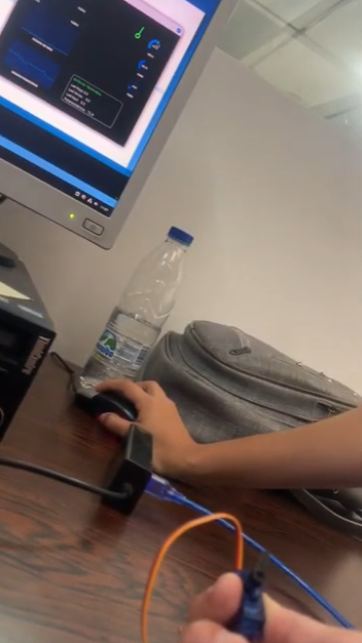
\includegraphics[width=0.4\linewidth]{img/resultado_act3_servo.png}
    \caption{Interfaz con el knob activo y el servo respondiendo al mismo \'{a}ngulo.}
    \label{fig:resultado_act3_servo}
\end{figure}

\clearpage
%%%%%%%%%%%%%%%%%%%%%%%%%%%%%%%%%%%%%%%%%%%%%%%%%%%%%%%%%%%%%%%%%%%%%%%
\section{Conclusiones}
Con estas actividades se pudo ver c\'{o}mo Firmata simplifica mucho el trabajo, ya que no
hay que reprogramar el Arduino cada vez que se quiere cambiar algo en la l\'{o}gica del
programa. Toda la parte de control queda en Processing y la placa solo obedece lo que
se le manda por serial.

En la actividad 5.2 se comprob\'{o} que mezclar colores en el LED RGB es directamente
proporcional al valor PWM de cada canal. El detalle de usar el alfa del color en los LEDs
virtuales funcion\'{o} bien para representar el brillo en pantalla de la misma forma que
en el f\'{i}sico.

En la actividad 5.3 se validó que la interfaz responde dinámicamente a los cambios del 
entorno. Al bloquear la luz sobre la fotorresistencia, la caída de valores en el gráfico 
y el cambio en la opacidad del LED virtual demostraron que se pueden procesar señales 
analógicas complejas de forma visual e intuitiva.

En la actividad 5.4 el truco del rango negativo en el knob ($-180$ a $0$) fue lo que
permiti\'{o} cumplir el requisito de que el centro coincida con $90^\circ$ en el servo,
simplemente negando el valor antes de mandarlo con \texttt{servoWrite()}~\cite{arduinoref}.

\clearpage
%%%%%%%%%%%%%%%%%%%%%%%%%%%%%%%%%%%%%%%%%%%%%%%%%%%%%%%%%%%%%%%%%%%%%%%
\begingroup
\small
\begin{thebibliography}{9}

\bibitem{firmata}
F.~Mellis, H.~Barragan y otros, ``Firmata Protocol Documentation,''
\emph{Firmata GitHub Repository}, 2006--2024.
[En l\'{i}nea]. Disponible: \url{https://github.com/firmata/protocol}.
[Consulta: jun.~2026]

\bibitem{arduinoref}
Arduino, ``Arduino Language Reference,'' \emph{Arduino Documentation},
Arduino LLC, 2024. [En l\'{i}nea]. Disponible:
\url{https://docs.arduino.cc/language-reference/}. [Consulta: jun.~2026]

\bibitem{controlp5}
A.~Cockpit, ``controlP5 --- A GUI Library for Processing,'' 2012--2023.
[En l\'{i}nea]. Disponible: \url{https://www.sojamo.de/libraries/controlP5/}.
[Consulta: jun.~2026]

\bibitem{guialab}
A.~Russoniello, ``Laboratorio: Interfaz Gr\'{a}fica con Processing y Protocolo Firmata,''
gu\'{i}a de pr\'{a}ctica de laboratorio, Laboratorio General (Internet de las Cosas),
Escuela de Computaci\'{o}n, Facultad de Ciencias,
Universidad Central de Venezuela, Caracas, 2026.

\end{thebibliography}
\endgroup

\end{document}
